\chapter{Qual é a chance?}
\markboth{Módulo 7}{}

\section*{Habilidades do SAEB}

\begin{itemize}
\item Identificar, entre eventos aleatórios, aqueles que têm menos, maiores ou
iguais chances de ocorrência, sem utilizar frações.

\item Determinar a probabilidade de ocorrência de um resultado em eventos
aleatórios, quando todos os resultados possíveis têm a mesma chance de
ocorrer (equiprováveis).
\end{itemize}

\subsection{Habilidade da BNCC}

\begin{itemize}
  \item 
 EF03MA25.
\end{itemize}

\conteudo{
Probabilidade é uma razão entre o que se espera ou se deseja que aconteça e o total
possível de possibilidades. Essa probabilidade indica
a chance de determinado resultado ocorrer. O número 0 representa uma
probabilidade de zero em cada cem, ou seja, chance nenhuma de o resultado ocorrer;
o número 1 corresponde à probabilidade cem em cada cem, o que quer
dizer que será certeza de que o evento ocorrerá.
}

\pagebreak 

\section*{Atividades}

\num{1} Em um estojo há 25 lápis coloridos e 18 lápis pretos. Retirando-se, ao
acaso, um lápis desse estojo, o que tem chance maior: retirar um lápis
colorido ou um lápis preto? Justifique sua resposta.
\reduline{Como há mais lápis coloridos do que pretos no estojo, a maior chance
quando se retira um único lápis desse estojo é a de que saia um lápis
colorido.\hfill}
%\reduline{Professor, aproveite o exercício para dar outros exemplos e, aos poucos,
%ir trabalhando o conceito com os alunos, devido à importância de eles
%desenvolverem essa habilidade de encontrar maiores chances por meio de uma análise simples.\hfill}

\num{2} Daniel joga um dado de seis faces, numeradas de 1 a 6, que não foi modificado e funciona perfeitamente. Calcule a probabilidade de Daniel passar pelas seguintes situações.

\begin{figure}[htpb!]
\centering
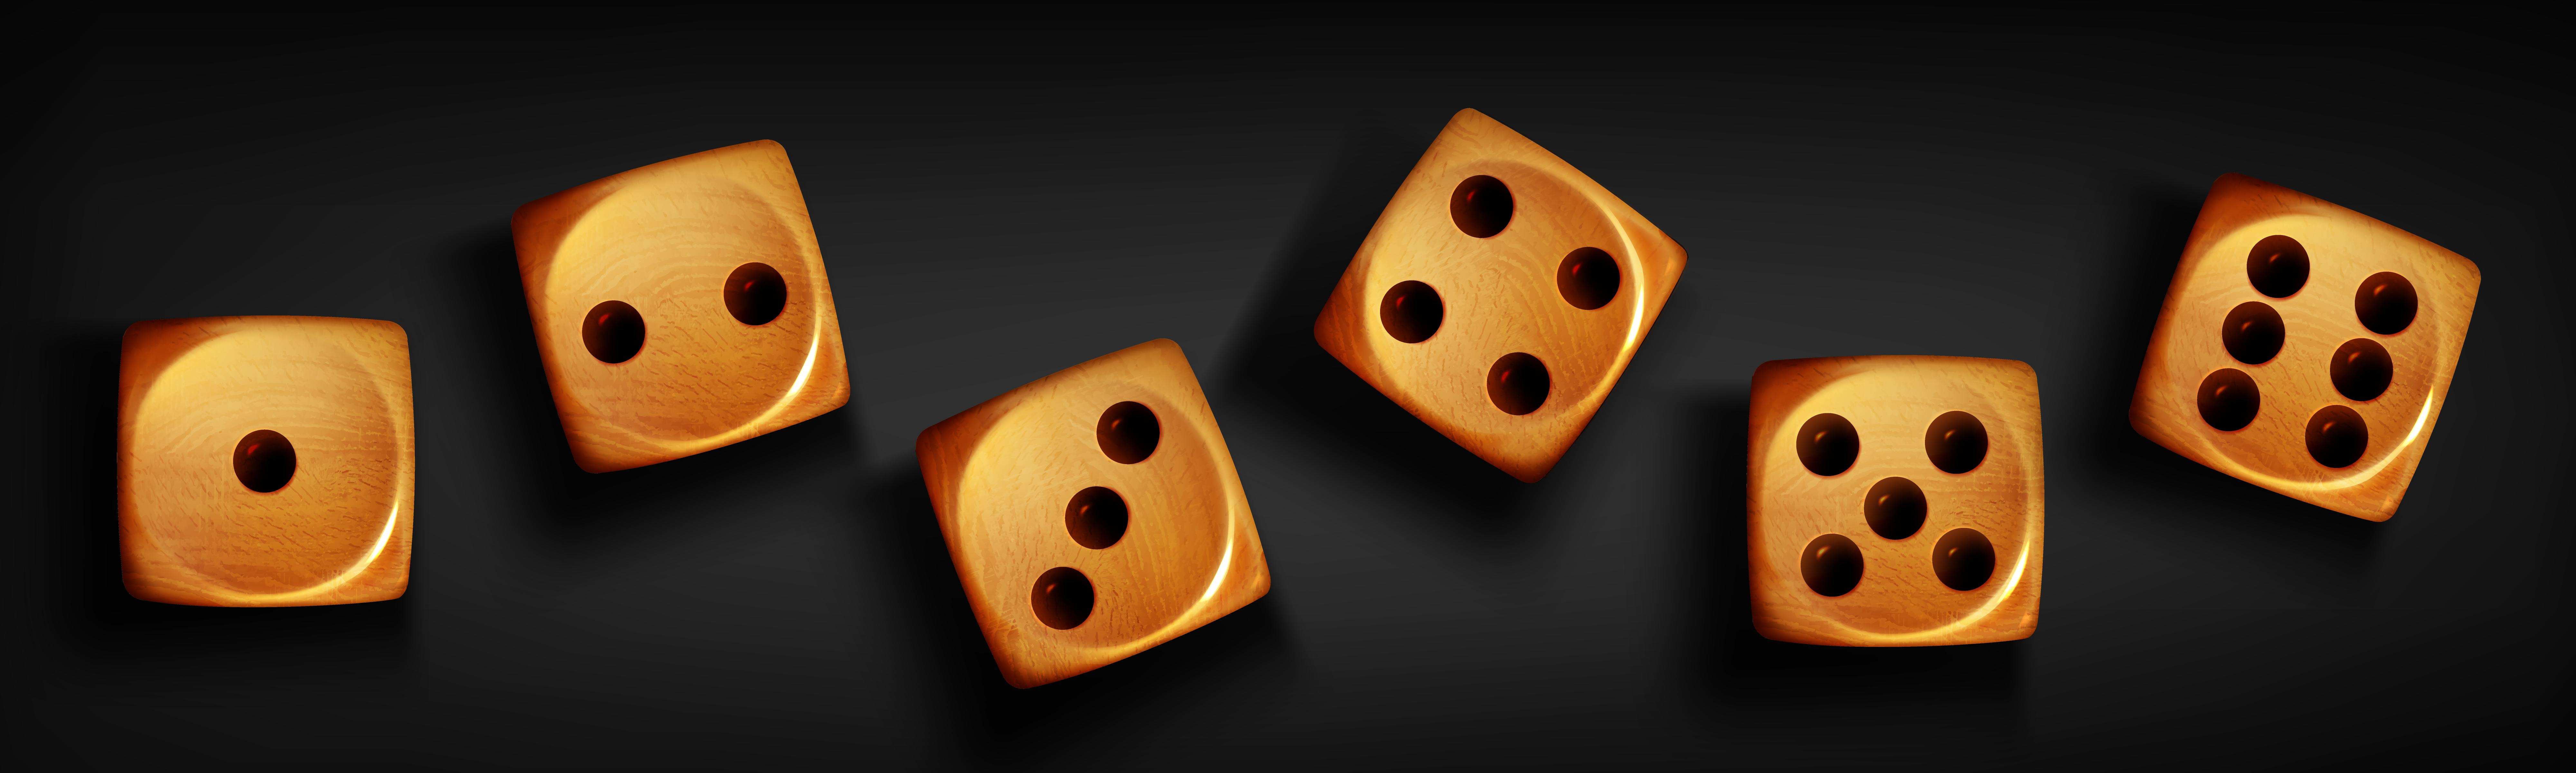
\includegraphics[width=0.8\textwidth]{./media/image75a.jpg}
\end{figure}

\begin{escolha}
\item Tirar, na face voltada para cima, um número par.
\reduline{Temos 6 possibilidades de números que podem sair: 1, 2, 3, 4, 5 e 6. Interessa, nesse caso, um número par: 2, 4 e 6. Portanto a probabilidade será de metade das chances, ou seja, de uma em cada duas.\hfill}

\item Tirar, na face voltada para cima, um número ímpar.
\reduline{Temos 6 possibilidades de números que podem sair: 1, 2, 3, 4, 5 e 6. Interessa, nesse caso, um número par: 1, 3 e 5. Portanto a probabilidade será de metade das chances, ou seja, de uma em cada duas.\hfill}

\item Tirar, na face voltada para cima, um número menor do que 3.
\reduline{Temos 6 possibilidades de números que podem sair: 1, 2, 3, 4, 5 e 6. Interessa, nesse caso, um número menor que 3: 1 e 2. Portanto a probabilidade é de uma em cada três.\hfill}
\end{escolha}

\num{3} Uma sacola escura, que não permite visualizar o que tem dentro, contém
20 bolas idênticas, mas de cores diferentes. Sabe-se que 6 são azuis, 8
são pretas, 4 são vermelhas e 2 são amarelas. Retirando-se uma bola ao
acaso:

\begin{escolha}
\item Qual cor de bola tem mais chances de sair?
\reduline{A maior chance é de sair uma bola preta.\hfill}
\linhas{1}

\item  Qual cor de bola tem menos chances de sair?
\reduline{A menor chance é de sair uma bola amarela.\hfill}
\end{escolha}

%\coment{Deixe bem claro que a probabilidade máxima de algo acontecer e 100 em cada cem, assim como a mínima é de zero em cada cem.}

\num{4} Lucas tem guardados, em uma caixa, 10 livros de matemática, 5 de história, 3 de inglês e
2 de geografia. Retirando-se um desses itens, ao acaso, da caixa,
responda:

\begin{figure}[htpb!]
\centering
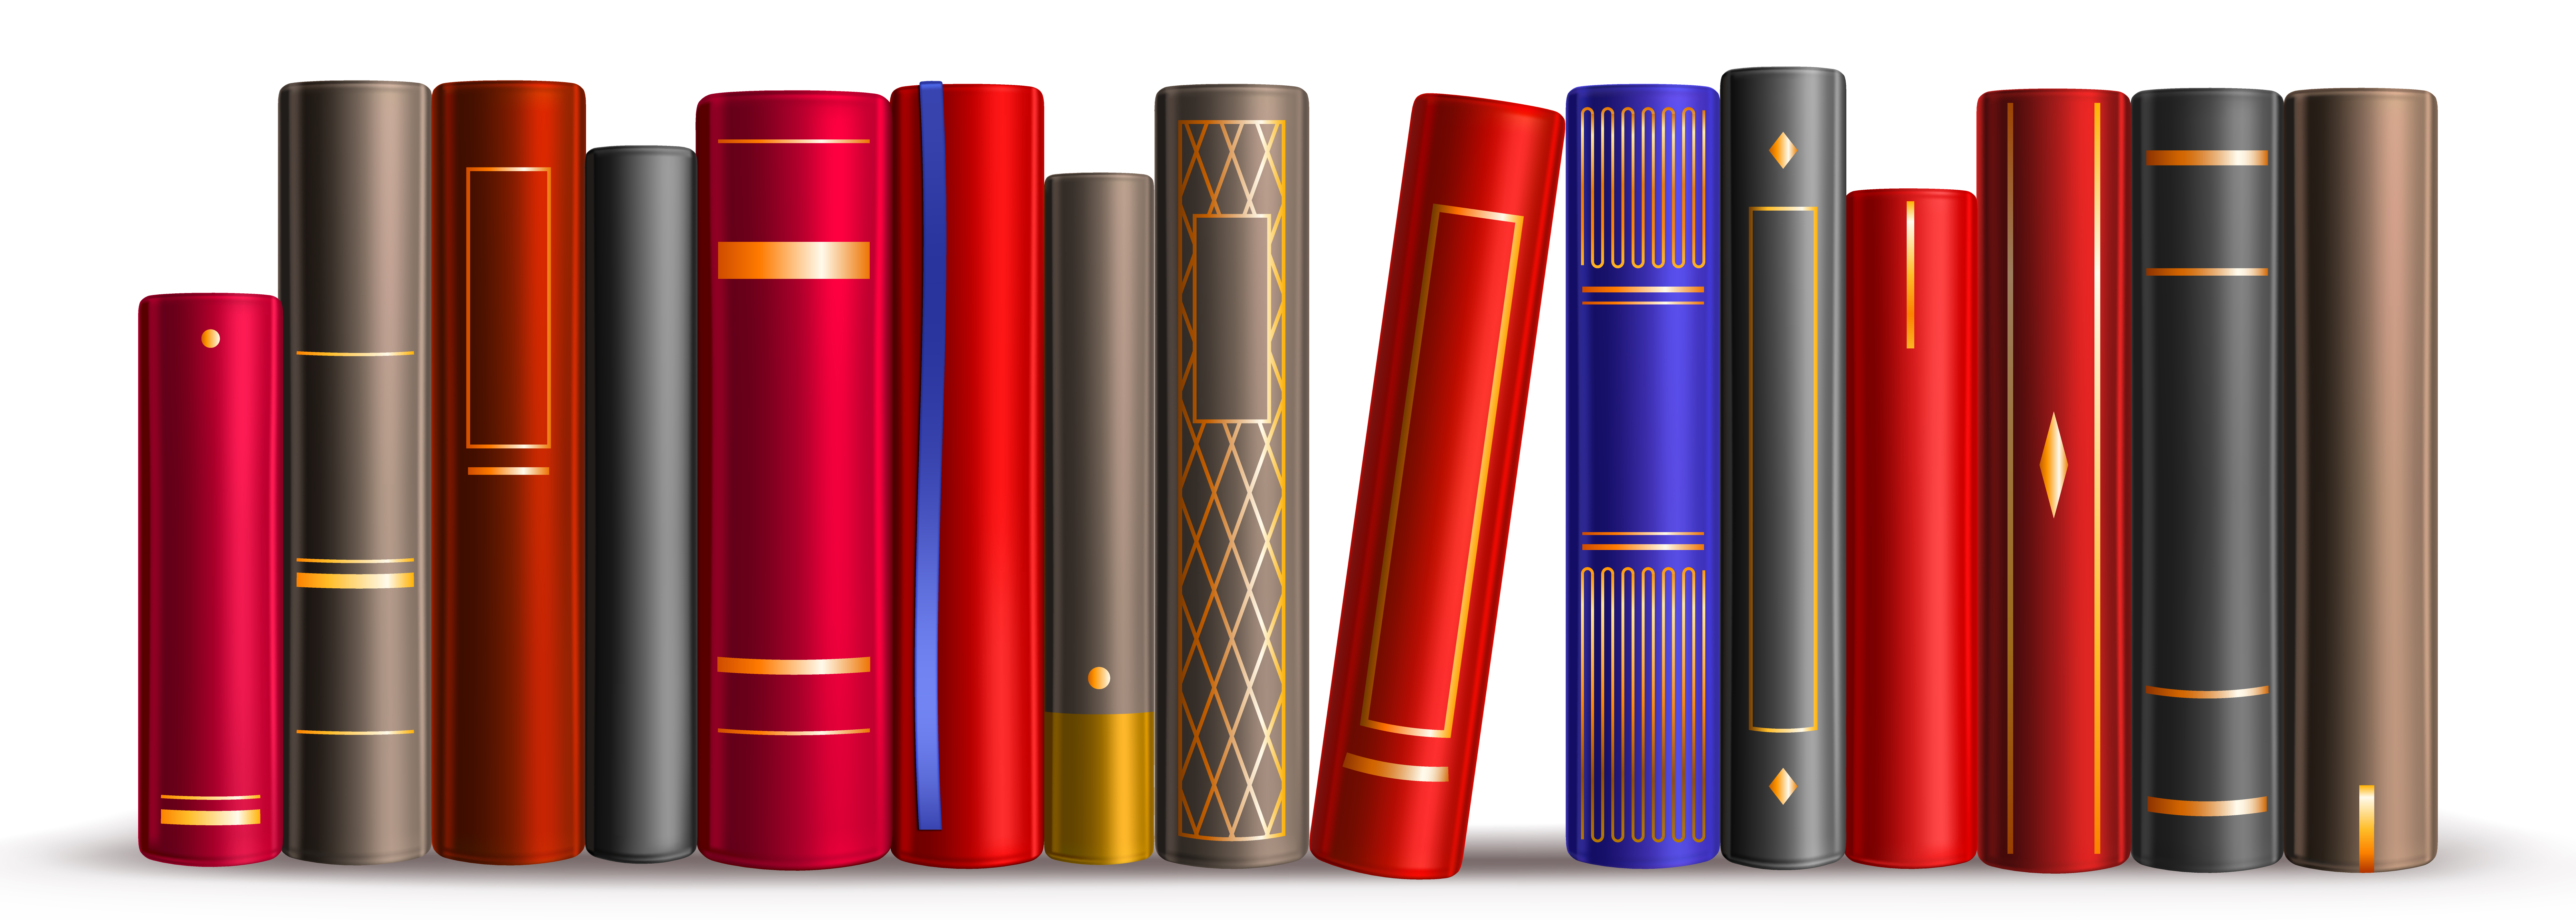
\includegraphics[width=0.8\textwidth]{./media/image75b.jpg}
\end{figure}

\begin{escolha}
\item Qual é a chance de ser um livro?
\reduline{A chance é total, ou seja, de 100 em 100, já que há apenas livros na caixa.\hfill}

\item  Qual é a probabilidade de ser um livro de matemática?
\reduline{A probabilidade é de 1 em cada 2, ou metade, ou 50 em cada 100.\hfill}
\end{escolha}

\num{5} Um baralho convencional é composto por 52 cartas divididas em quatro
naipes (copas, paus, ouros e espadas), sendo 13 de cada naipe. Dessa
forma, se retirarmos uma carta ao acaso, qual a probabilidade de sair
uma carta do naipe de copas?

\begin{figure}[htpb!]
\centering
\includegraphics[width=\textwidth]{./media/image75c.jpg}
\end{figure}

\reduline{Total de cartas de um baralho comum: 52. Total de cartas de copas: 13. Probabilidade = 13 em 52 = uma em cada quatro.\hfill}

\num{6} Na sala em que Clarissa estuda há 32 alunos, dos quais 8 são meninas. A
professora irá escolher um aluno para verificar se este fez a tarefa.
Qual a probabilidade de um menino ser escolhido?
\reduline{Total de alunos: 32. Número de meninos: 32 - 8 = 24. Portanto, a probabilidade será de 24 em cada 32, ou seja, 3 em cada 4.\hfill}

\num{7} Uma letra é escolhida ao acaso dentre as que formam a palavra
FUNDAMENTO. A probabilidade de essa letra ser uma vogal é maior ou menor do que a de ser uma consoante?
\reduline{Total de letras: 10. Total de vogais: 4; total de consoantes: 6. Portanto, a probabilidade de ser uma vogal é menor do que a de ser uma consoante.\hfill}

\num{8} Vítor quer escolher um número para sua camiseta do time de futebol e ele
pode escolher qualquer número de 1 a 16. Qual a probabilidade de que ele
escolha um número maior que 8 e menor que 14?

\begin{figure}[htpb!]
\centering
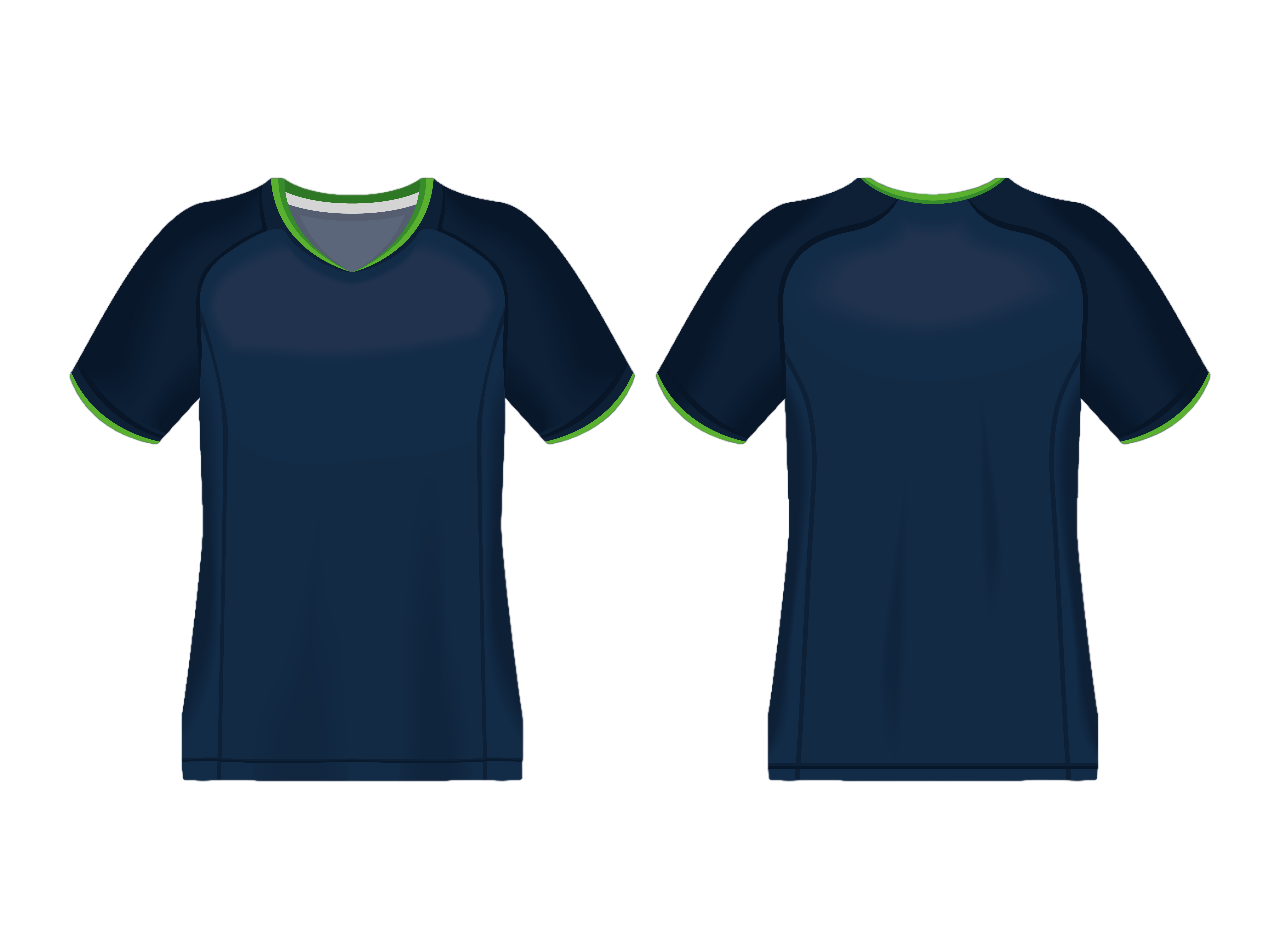
\includegraphics[width=0.7\textwidth]{./media/image75d.png}
\end{figure}

\reduline{Total de números: 16. Total de números que interessam: 5, sendo eles 9, 10, 11, 12 e 13. Probabilidade de 5 em 16.\hfill}
\linhas{1}

\num{9} Os 450 estudantes de um colégio responderam a uma pergunta sobre qual a
sua área de conhecimento preferida, entre Exatas, Humanidades e
Biológicas. As respostas foram computadas e alguns dados foram colocados
na tabela.

\vspace{2ex}

\begin{longtable}[]{@{}ll@{}}
\toprule
\hline
\textbf{Área} & \textbf{Sexo Masculino (M)}\tabularnewline
\hline
\textbf{Exatas (E)} & 200\tabularnewline
\hline
\textbf{Humanas (H)} & 150\tabularnewline
\hline
\textbf{Biológicas (B)} & 100\tabularnewline
\hline
\textbf{Total} & 265\tabularnewline
\hline
\bottomrule
\end{longtable}

\pagebreak
Um estudante é escolhido ao acaso. Determine a probabilidade de esse
estudante preferir humanas.
\reduline{Total de estudantes: 450. Preferência por humanas: 150. Probabilidade: 450/150 = 3 = uma chance em cada três.\hfill}
\linhas{3}


\num{10} Carlos possui duas urnas com bolas que só são diferenciadas pela cor. A
distribuição das bolas nas urnas e por cor se encontra na tabela a
seguir.

\begin{longtable}[]{@{}lll@{}}
\toprule
\hline
\textbf{Cor} & \textbf{Urna 1} & \textbf{Urna 2}\tabularnewline
\hline
\midrule
\endhead
Amarela & 4 & 0\tabularnewline
\hline
Azul & 3 & 1\tabularnewline
\hline
Branca & 2 & 2\tabularnewline
\hline
Verde & 1 & 3\tabularnewline
\hline
Vermelha & 0 & 4\tabularnewline
\hline
\bottomrule
\end{longtable}


Ele irá colocar todas as bolas dessas duas urnas em uma única urna 3. Em
seguida retirará uma bola, ao acaso, dessa última urna. Qual a
probabilidade de que ele retire uma bola verde?
\reduline{Total de bolas: 20. Bolas verdes: 4. Probabilidade: 4 em cada 20, ou 1 em cada 5, ou 25 em cada 100.\hfill}
\linhas{6}

\pagebreak
\section*{Treino}

\num{1} Mateus tem uma coleção de carrinhos em miniatura. No total, ele tem 30 carrinhos, sendo 10 caminhões (metade deles com 4 rodas e a outra metade com 6 rodas), 15 carrinhos conversíveis e 5 jipes. Se ele pegar um dos carrinhos de olhos fechados, sem escolher, para dar de presente ao seu irmão, quais são as chances de ser um caminhão de 6 rodas?

\begin{figure}[htpb!]
\centering
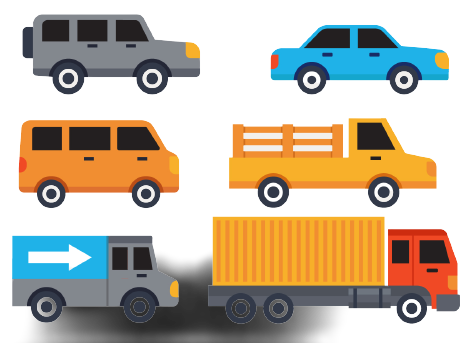
\includegraphics[width=0.4\textwidth]{./media/image75f.png}
\end{figure}

\begin{escolha}
\begin{multicols}{2}
\item
  dez em cada trinta.
\item
  cinco em cada trinta.
\item
  um em cada trinta.
\item
  trinta em cada trinta.
\end{multicols}
\end{escolha}


\num{2} Em uma festa à fantasia, cujo tema é alimentação, estiveram presentes  100 convidados com as seguintes fantasias:

\begin{myquote}
\begin{itemize}
  \begin{multicols}{2}
\item [] Maçã: 12
\item [] Batata frita: 20
\item [] Cacho de uva: 8
\item [] Frango assado: 31
\item [] Bolacha: 9
\item [] Bolo: 7
\item [] Kiwi: 10
\item [] Cachorro-quente: 3
  \end{multicols}
\end{itemize}
\end{myquote}

Se uma dessas pessoas for escolhida, aleatoriamente, para ganhar um prêmio, qual a chance de ela estar fantasiada de fruta?

\begin{escolha}
\begin{multicols}{2}
\item
30 em cada 100.
\item
50 em cada 100.
\item
Nenhuma chance.
\item
Chance total, de 100 em cada 100.
\end{multicols}
\end{escolha}


\num{3} Uma turma de terceiro ano tem 23 alunos.~Três deles, Ana, Carlos e Tatiana, candidataram-se para serem representantes de turma. Nessa votação, cada aluno só pode votar uma vez, e os candidatos não votam. Veja a lista de chamada, com os primeiros nomes dos alunos, dessa turma.

\begin{myquote}
\begin{multicols}{3}
\begin{enumerate}
\item [] Abigail

\item [] Ana

\item [] Aparecida

\item [] Bernardo

\item [] Carla

\item [] Carlos

\item [] Coralina

\item [] Daniel 

\item [] Elena

\item [] Estêvão

\item [] Gustavo

\item [] Helena

\item [] Hilda

\item [] Ingrid

\item [] Janaína

\item [] Joaquim

\item [] Juarez

\item [] Manuel

\item [] Nina

\item [] Paula

\item [] Pedro

\item [] Rafael

\item [] Tatiana
\end{enumerate}
\end{multicols}
\end{myquote}

Imagine que a professora sorteie um aluno, de forma aleatória, para ser o primeiro a votar. Quais as chances de esse primeiro votante ter o nome iniciado com a mesma letra de um dos nomes dos candidatos?

\begin{escolha}
\begin{multicols}{2}
\item
3 em 20.
\item
4 em 20.
\item
7 em 20.
\item
Nenhuma chance.
\end{multicols}
\end{escolha}

